\section*{Введение}

Современная , однако одтельные области машинного обучения развиваются медленно или недостаточно быстро.

\begin{figure}[!ht]
\centering
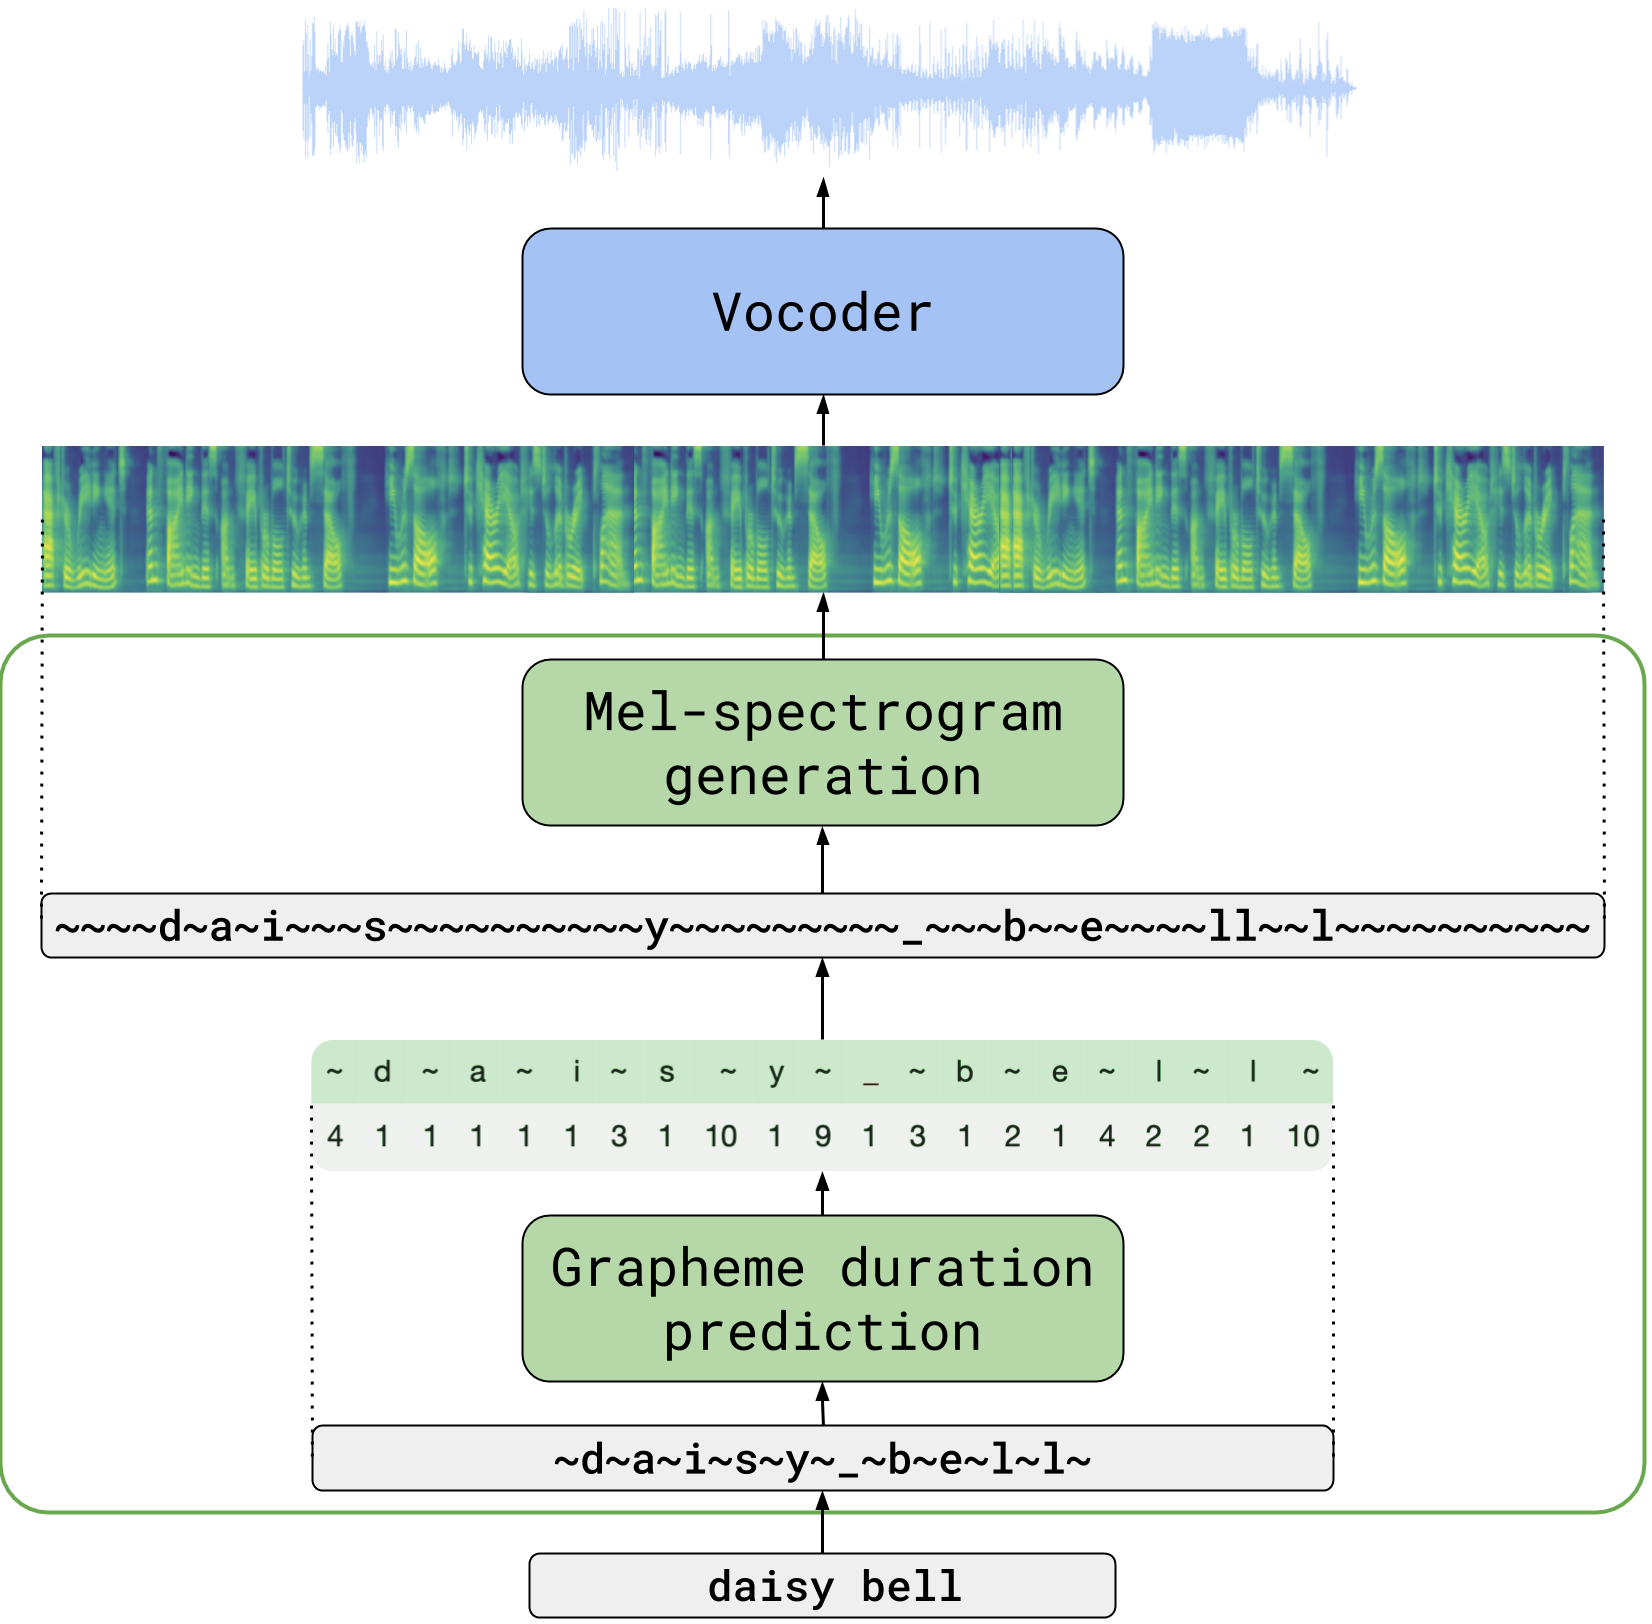
\includegraphics[width=1.0\textwidth]{images/arch.png}
\caption{TalkNet converts text to speech, using a grapheme duration predictor, a mel-spectrogram generator, and a vocoder. We use $\sim$ to denote the CTC blank symbol.}
\label{fig:arch}
\end{figure}

Таким образом, целью данной работы является разработка модели машинного обучения, позволяющей производить эффективную, качественную и быструю генерацию речи из входного текста. В рамках данной работы, решение будет основываться на сверточных (конволюционных) сетях с неавторегрессионной архитектурой, позволяющей расчитывать на максимальную производительность на современных графических ускорителях (GPU).

Для достижения описанной выше цели необходимо решить следующие задачи:
\begin{itemize}
    \item Проанализировать предметную область и существующие модели. Обозначить основные проблемы и пути к их решению.
    \item Разработать и описать эффективную архитектуру, основанную на идеи неавторегрессионности.
    \item Выбрать данные для обучения и провести эксперименты.
    \item Произвести сравнение подходов и анализ результатов на качество и скорость.
\end{itemize}

В рамках данной работы мы предлагаем TalkNet: сверточную неавторегрессионную нейронную модель для задачи синтеза речи. Модель состоит из двух прямых (feed-forward) полностью сверточных сетей. Первая сеть предсказывает длительность входных символов (графем), выравнивая таким образом входную последовательность на длинну мэл-спеткрограммы. Далее, производится операция расширения (expansion) входного текста путем повторения каждого символа в соответствии с предсказанной длительностью. Вторая сеть генерирует мэл-спектрограмму из развернутого текста. Операция разворачивания, таким образом, позволяет построить неавторегрессионную архитектуру.

Чтобы обучить предиктору длительности графемы, мы добавляем длительность графемы в обучающий набор данных, используя предварительно обученную модель распознавания речи на основе Коннекционистской временной классификации (CTC). Явное предсказание длительности исключает пропуск и повторение слов. Эксперименты с набором данных речи ЖЖ показывают, что качество речи почти соответствует авторегрессионным моделям. Модель очень компактна - она имеет параметры 10,8 м, что почти в 3 раза меньше, чем современные модели преобразования текста в речь. Неавторегрессионная архитектура позволяет быстро обучаться и делать выводы.
\sep
To train a grapheme duration predictor, we add the grapheme duration to the training dataset using a pre-trained Connectionist Temporal Classification (CTC)-based speech recognition model. The explicit duration prediction eliminates word skipping and repeating. Experiments on the LJSpeech dataset show that the speech quality nearly matches auto-regressive models. The model is very compact -- it has 10.8M parameters, almost 3x less than the present state-of-the-art text-to-speech models. The non-autoregressive architecture allows for fast training and inference.

В главе $1$ будут описана формальная постановка задачи генерации речи и существующие подходы к ее решению, а также их недостатки и достоинства. В главе $2$ происходит описание главной идеи TalkNet с разбиением процесса генерации на два шага. Глава $3$ посвящена описанию данных и проводимых экспериментов, а также подробностях процесса обучения. В главе $4$ проводится анализ результатов с точки зрения качества и скорости.